\begin{formula}{Wichtige Folgen}\\
    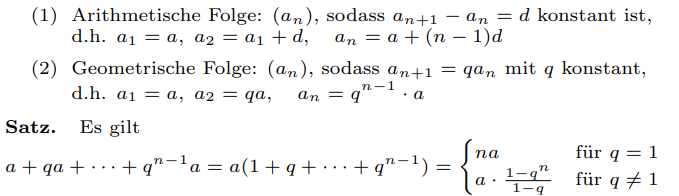
\includegraphics[scale=0.5]{Analysis1/zsf/Images/Folgen_Reihen/wichtige_folgen.png}
\end{formula}
\begin{remark}
    Folgend sind diese Konzepte beispielhaft vereinfacht.\\
    Abkürzungen
    \begin{itemize}
      \item $A=$ Anfangs-Glied
      \item $d=$ Differenz
      \item $q=$ Quotient
    \end{itemize}
\end{remark}

\begin{definition}{Arithmetische Folge}
$$
a_{k}=(2,3,4,5, \ldots) \rightarrow d=1, A=2
$$

N-tes Glied

$$
a_{n}=A+(n-1) \cdot d
$$

Mittelwert

$$
a_{k}=\frac{a_{k-1}+a_{k+1}}{2}
$$

Partial-Summe

$$
S_{n}=n \cdot \frac{a_{1}+a_{n}}{2}=n \cdot\left(A+\frac{n-1}{2} \cdot d\right)
$$
\end{definition}

\begin{definition}{Geometrische Folge}
$$
a_{k}=\left(\frac{1}{1}, \frac{1}{2}, \frac{1}{4}, \frac{1}{8}, \ldots\right) \rightarrow q=\frac{1}{2}, A=1
$$

N-tes Glied
$$a_{n}=A \cdot q^{n-1}=\frac{A}{q} \cdot q^{n}$$

Mittelwert
$$
\left|a_{k}\right|=\sqrt{a_{k-1} \cdot a_{k+1}}
$$

Partial-Summe

$$
S_{n}=A \cdot \frac{1-q^{n}}{1-q}=A \cdot \frac{q^{n}-1}{q-1}
$$
\end{definition}